\section{Results}
\label{sec:results}

The data cover 165 conditions, 23,104 replicas, 17,474 exits and 30 saddles.
\Tabref{tab:verdicts} gives the verdict on each claim, and the rest of this section gives the evidence.

\begin{table}[t]
    \centering
    \caption{Verdicts on each numerical claim. Ranges in brackets are 95\% confidence intervals. Unless noted, values are for \fmnist. $k$ statistics cover 28 conditions.}
    \label{tab:verdicts}
    \resizebox{\textwidth}{!}{%
    \begin{tabular}{@{}lll@{}}
        \toprule
        \textbf{Claim} & \textbf{Verdict} & \textbf{Key measurement} \\
        \midrule
        Weibull, not exponential & Partly & $k=1$ rejected in 86\%; Weibull best by AIC in 4 of 28 \\
        $k$ between 0.7 and 1.3 & Refuted & 32\% in range; median 1.47, maximum 3.33 \\
        $k$ depends on geometry & Refuted & $\rho(k,\log\lmax)=-0.06$, $p=.77$ \\
        \midrule
        Adam 2--5$\times$ faster at narrow basins & Partly & 2.75$\times$ [1.89, 5.18]; 2.01$\times$ with medians observed \\
        Adam similar at wide basins & Refuted & 1.89$\times$ [1.24, 3.22]; no significant narrow/wide difference \\
        \midrule
        Doubling $B$ multiplies $\tau$ by $\sqrt{2}$ & Refuted & $\times$5.1 [3.4, 8.0]; slope 2.02 [1.64, 2.41], against 0.5 \\
        $\etaB$ controls temperature & Supported on \fmnist & Equal-ratio $\tau\eta$ within about 10\%; \digitsdata inconclusive (cap) \\
        \midrule
        Top eigenvector predicts exit, 70--85\% & Noise-dependent & 54\% at high noise, 82--86\% at lower noise ($r=1$) \\
        Eigenvalue gap predicts accuracy & Refuted & $\rho$ from $-0.07$ to $+0.23$, all n.s. \\
        \bottomrule
    \end{tabular}
    }
\end{table}


\subsection{Validation against Kramers}
\label{sec:validation}

{\bf Can the instrument recover a known answer?}
Yes.
At barrier-to-temperature ratio $\Delta/T\ge4$, measured $\tau$ over the exact Kramers time is 1.03--1.13 (median 1.07) across three well widths (\figref{fig:validation}).
Weibull $k$ falls from 1.18 at $\Delta/T=1$ to 1.00 at $\Delta/T=6$ when starting at the minimum.
A near-stationary start still gives 1.10 at $\Delta/T=1$, so part of the low-barrier excess is not start-up delay.

\begin{figure}[t]
    \centering
    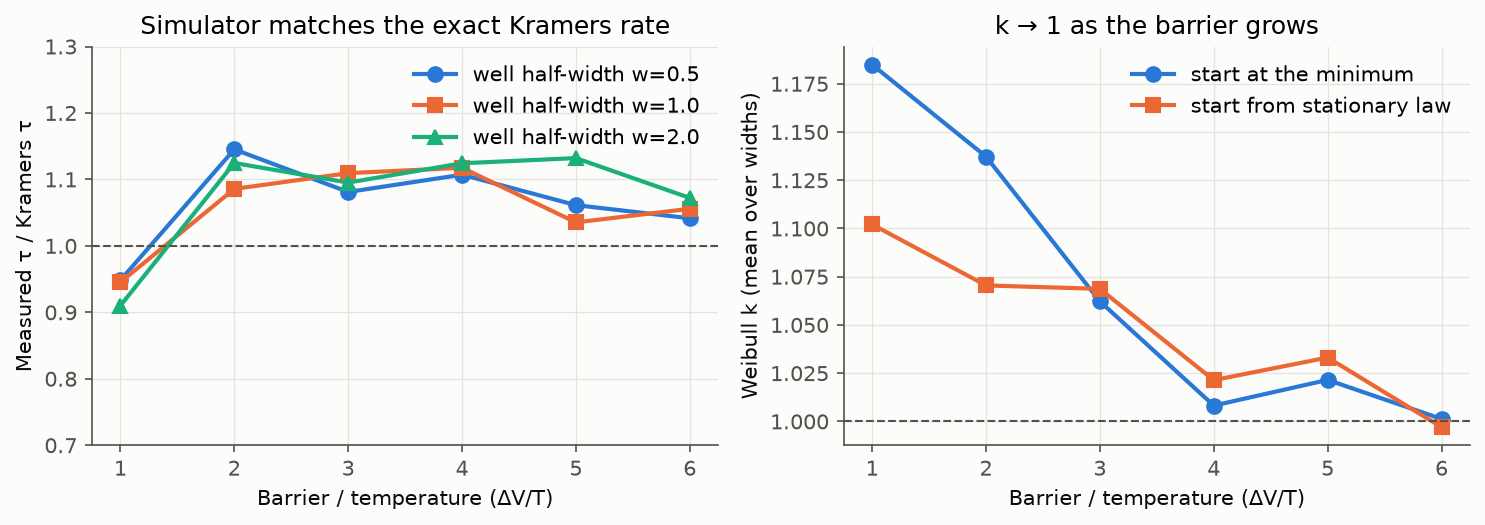
\includegraphics[width=0.95\linewidth]{figures/fig1_e0_validation.png}
    \caption{Validation on the controlled double well. \figleft{} Measured escape time over the exact Kramers time stays within 1.03--1.13 at $\Delta/T\ge4$ for three well widths. \figright{} Weibull $k$ approaches 1 as the barrier grows, the Poisson limit Kramers theory predicts. A start at the minimum adds more excess $k$ than a near-stationary start.}
    \label{fig:validation}
\end{figure}

\subsection{What escape looks like}
\label{sec:hops}

Exits are discrete hops.
In a typical condition, a replica lands on one of a few specific neighbours (median 3 distinct destinations by loss, and the top destination takes a median 88\% of exits).
The median condition has 89\% of exits landing at lower loss and 100\% crossing a barrier.
At the same $(\eta,B)$, $\tau$ across minima spans 550 to more than 150,000 steps.
A Newton audit of 192 accepted exits found 100\% strict minima and 98.4\% distinct from $\tstar$ (residual false exits 1.6\%, Wilson CI 0.5--4.5\%).
A same-seed GPU rerun of one condition reproduced every replica's exit check.

\subsection{H1: distribution shape}
\label{sec:h1}

{\bf Are escape times exponential?}
No (\tabref{tab:shape}).
{\bf Are they Weibull with $k$ in 0.7--1.3?}
Also no.
The likelihood-ratio test rejects $k=1$ in 86\% of conditions, but only 32\% of $k$ values lie in the hypothesized range, and 68\% exceed 1.3 (\figref{fig:distributions}).
Geometry does not explain the spread: $k$ is uncorrelated with $\log\lmax$, $\log$ trace and $\log$ det.

\begin{table}[t]
    \centering
    \caption{Distribution shape across the 28 E1 conditions with at least 50\% exits. Criteria failures in \textbf{bold}.}
    \label{tab:shape}
    \resizebox{\textwidth}{!}{%
    \begin{tabular}{@{}llll@{}}
        \toprule
        \textbf{Statistic} & \textbf{Value} & \textbf{Criterion} & \textbf{Met?} \\
        \midrule
        Likelihood-ratio test rejects $k=1$ (FDR 5\%) & 86\% & majority & Yes \\
        $\Delta$AIC(Weibull $-$ exponential) $<-10$ & 75\% & majority & Yes \\
        $k$ within 0.7--1.3 & 32\% & $\ge$90\% & \textbf{No} \\
        $k<1$ / $k>1.3$ & 11\% / 68\% & both present & Yes \\
        $k$ range (median) & 0.79--3.33 (1.47) & -- & -- \\
        Spearman $k$ vs $\log\lmax$ / $\log$ trace / $\log$ det & $-0.06$ / $-0.08$ / $-0.20$ & $p<.05$ & \textbf{No} ($p=.77$/$.68$/$.31$) \\
        \bottomrule
    \end{tabular}
    }
\end{table}


Weibull is also not singled out.
The best AIC model is lognormal in 13 conditions, gamma in 8, Weibull in 4 and shifted exponential in 3.
Across these 28 conditions, gamma beats Weibull by a median 5.1 AIC units and lognormal beats it by 6.4, while Weibull beats shifted exponential by 6.9.
Adam shows the same pattern: on \fmnist, median $k$ is 1.50 and 22\% of the 32 conditions with at least 50\% exits lie in range.
Excluding the 8 conditions with fewer than 50\% exits removes minima that barely escape, so we do not observe tail behaviour there.

\begin{figure}[t]
    \centering
    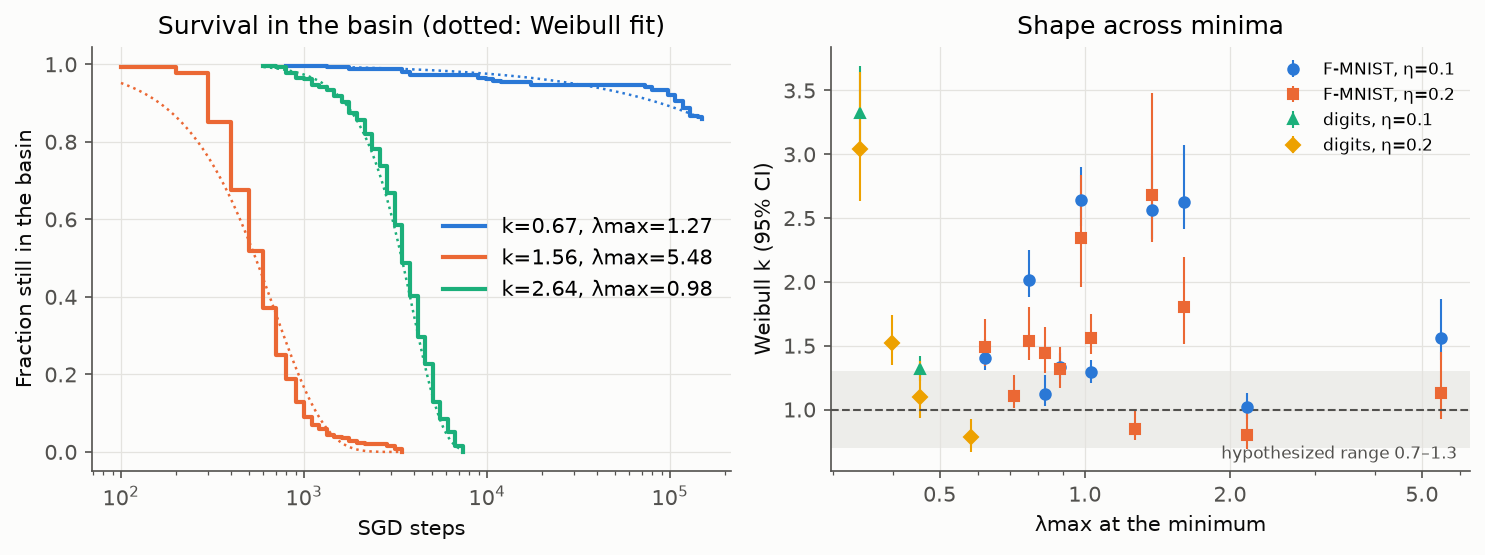
\includegraphics[width=0.95\linewidth]{figures/fig2_distributions.png}
    \caption{Distribution shape. \figleft{} Survival curves at three minima with Weibull fits (dotted). The $k=0.67$ minimum has only 14\% exits, so it is outside the 28 conditions in \tabref{tab:shape}. \figright{} Weibull $k$ against $\lmax$. Most values lie above the hypothesized band, and no trend with $\lmax$ appears.}
    \label{fig:distributions}
\end{figure}

\para{Why $k\ne1$.}
Two mechanisms account for most of the deviation.
{\em Delay:} discarding the first 25\% of exits and refitting residual time gives median $k=1.03$ (IQR 0.90--1.20), and 50\% of conditions fall within 0.85--1.15, against 18\% before truncation.
Discarding 50\% gives 1.05.
{\em Heterogeneity:} pooling minima gives $k=0.74$ and 0.59 on \fmnist and 0.52 and 0.57 on \digitsdata, against within-minimum means of 1.76, 1.51, 2.32 and 1.61.
Pooling alone flips the sign of $k-1$.
Escape is still not fully memoryless after the delay.
Hazards rise and then fall late (\figref{fig:hazard}), and residual $k$ still ranges from 0.74 to 1.79, so a constant hazard after a delay is only an approximation.

\begin{figure}[t]
    \centering
    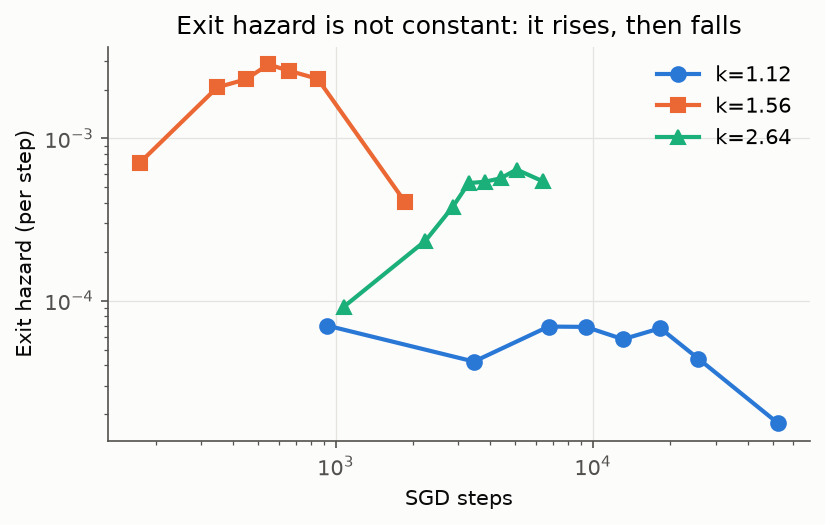
\includegraphics[width=0.55\linewidth]{figures/fig3_hazard.png}
    \caption{Exit hazard at three minima. The hazard rises during the early delay and falls late, including at minima with very different $k$. A Weibull with $k>1$ cannot show the late fall.}
    \label{fig:hazard}
\end{figure}

\subsection{H2: Adam against SGD}
\label{sec:h2}

{\bf Is Adam faster at narrow basins only?}
No.
At matched in-basin loss, Adam is about twice as fast across the board, with no demonstrated dependence on width (\tabref{tab:adam}, \figref{fig:adam}).
The narrow point estimate of 2.75 is in the hypothesized range, but its interval [1.89, 5.18] is wider than [2, 5], so H2a fails its criterion.
H2b fails because the wide ratio is 1.89 and its interval excludes 1.
H2c is not significant: the narrow/wide ratio is 1.46 [0.74, 3.09], and the Spearman correlation of ratio with $\log\lmax$ is 0.47 ($p=.12$).
With $n=12$ we cannot exclude a moderate effect.
Keeping only minima with observed medians brings narrow and wide nearly level, at 2.01 and 1.91.
On \digitsdata the ratio is 1.56 [0.90, 3.22], with 5 of 6 minima involving a censored median, so this is weak evidence.

\begin{table}[t]
    \centering
    \caption{Adam against SGD on \fmnist. \emph{Top:} $\tau_{\text{SGD}}/\tau_{\text{Adam}}$ at matched in-basin loss. The last column keeps only minima where all medians are observed; capped medians make the others bounds. \emph{Bottom:} ablations on 6 minima, as $\tau/\tau_{\text{SGD}}$ at $\eta=0.1$. One of the 6 has a capped SGD median, so the second column drops it. Main estimates in \textbf{bold}.}
    \label{tab:adam}
    \resizebox{\textwidth}{!}{%
    \begin{tabular}{@{}lccc@{}}
        \toprule
        \textbf{Group} & \textbf{Ratio, all minima} & \textbf{95\% CI} & \textbf{Observed only} \\
        \midrule
        Narrow (top third by $\lmax$, $n=4$) & \textbf{2.75} & 1.89--5.18 & 2.01 ($n=3$) \\
        Wide (bottom third, $n=4$) & \textbf{1.89} & 1.24--3.22 & 1.91 ($n=3$) \\
        Narrow/wide ratio & 1.46 & 0.74--3.09 & -- \\
        All minima ($n=12$) & 2.42 & 1.83--3.27 & 1.97 [1.56, 2.53] ($n=8$) \\
        \midrule
        \textbf{Ablation} & $\boldsymbol{\tau/\tau_{\text{SGD}}}$ \textbf{(6 minima)} & \textbf{95\% CI} & \textbf{Observed only} \\
        \midrule
        \rmsprop, lr 0.008, no momentum & 0.41 & 0.25--0.63 & 0.50 ($n=5$) \\
        Adam warm-started, lr 0.008 & 0.35 & 0.22--0.53 & 0.41 ($n=5$) \\
        \sgdm, same effective $\eta$ & 1.00 & same median check & 1.00 ($n=5$) \\
        Adam default lr 0.001 (5 minima) & No exits & -- & $\ge$ 7--34$\times$ slower ($n=4$) \\
        \bottomrule
    \end{tabular}
    }
\end{table}


\begin{figure}[t]
    \centering
    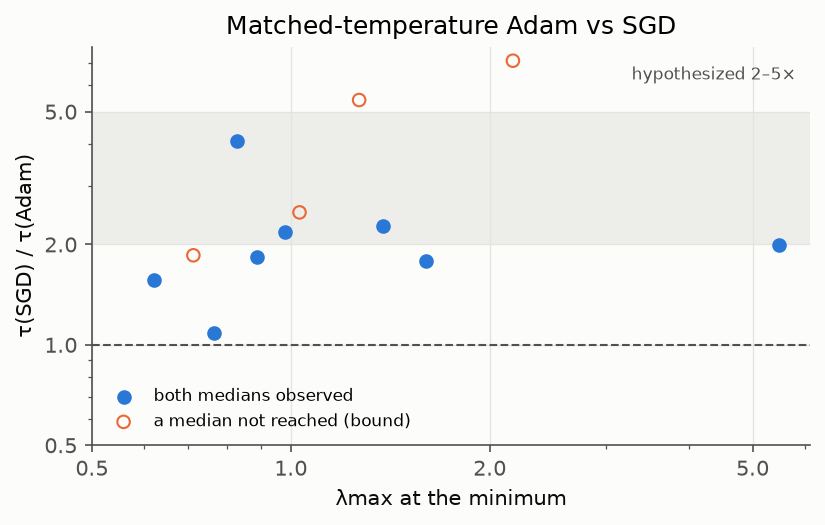
\includegraphics[width=0.55\linewidth]{figures/fig4_adam_sgd.png}
    \caption{Adam speed-up against $\lmax$ on \fmnist, at matched in-basin loss. Every minimum has ratio above 1, and the spread shows no clear trend with sharpness. Open markers involve a censored median and are bounds.}
    \label{fig:adam}
\end{figure}

\para{Ablations.}
\rmsprop reproduces Adam's speed-up without momentum, while \sgdm at the same effective $\eta$ lands on the same median check as SGD at all 6 minima (resolution about 10\%).
So the adaptive scaling is the source, and warm-starting Adam shows that it is not a cold-start artefact.
Calibration can reverse the direction: at its default learning rate of 0.001, Adam made no exits in 150,000 steps at 5 of 5 tested minima.
That is at least 7--34$\times$ slower than SGD at the 4 minima where SGD's median is observed.

In the double well with theory-matched Adam, $\tau_{\text{SGD}}/\tau_{\text{Adam}}$ is 0.68--0.80 in narrow wells and 0.87--1.27 in wide wells.
So Adam shows no consistent speed-up on a single barrier, even with curvature-aligned noise.
The network speed-up is therefore not a generic property of adaptive scaling, and we did not test its cause.

\subsection{H3: batch size and temperature}
\label{sec:h3}

{\bf Does doubling $B$ multiply $\tau$ by $\sqrt{2}$?}
No.
The factor is 5.1 [3.4, 8.0] on \fmnist, and the slope is 2.02 [1.64, 2.41] against the predicted 0.5, with per-minimum slopes of 1.5--2.8 (\tabref{tab:batch}, \figref{fig:batch}).
The structural part of H3 does hold: within the observed range, a power law in $B$ fits better than $\log\tau$ linear in $B$.
This comparison needs care.
It uses uncensored medians only, and Arrhenius predicts its fastest growth at large $B$, exactly where censoring removes data.
The falling step factors could also reflect only fast minima surviving to large $B$.
So our data favour a power law within the observed range, which is mostly $B=4$--32, and they do not rule out Arrhenius behaviour in general.
In E0, a single barrier, $\log\tau$ stays linear in $1/T$ even with loss-proportional noise, so that noise alone does not explain the network law.

\begin{table}[t]
    \centering
    \caption{Batch-size scaling at $\eta=0.1$. The hypothesis predicts slope 0.5 and factor 1.41. Lower AIC is better, and the preferred form is in \textbf{bold}. Fits use uncensored medians only.}
    \label{tab:batch}
    \resizebox{\textwidth}{!}{%
    \begin{tabular}{@{}lll@{}}
        \toprule
        \textbf{Measure} & \textbf{\fmnist (6 minima)} & \textbf{\digitsdata (3 minima)} \\
        \midrule
        Slope of $\log_2\tau$ on $\log_2 B$ & \textbf{2.02} [1.64, 2.41] & 3.4 (one minimum) \\
        $\tau$ factor per doubling & \textbf{5.1} [3.4, 8.0] & 18 [10, 41] \\
        Factor by step: $B=$ 4$\to$8 / 8$\to$16 / 16$\to$32 / 32$\to$64 & 5.9 / 3.8 / 4.2 / 2.4 & 23 / 5.1 / censored / censored \\
        AIC: power law vs Arrhenius & \textbf{$-$16.7} vs $+$16.1 & \textbf{$-$2.9} vs $+$6.4 \\
        \bottomrule
    \end{tabular}
    }
\end{table}


\begin{figure}[t]
    \centering
    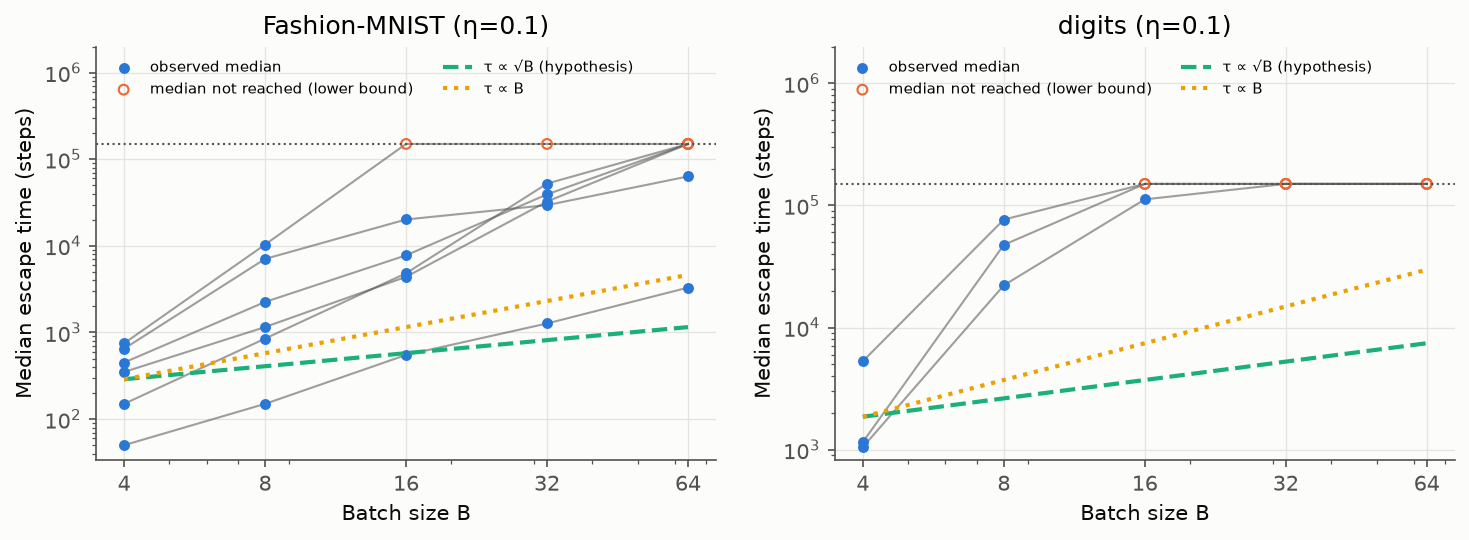
\includegraphics[width=0.95\linewidth]{figures/fig5_batch_scaling.png}
    \caption{Median escape time against batch size at $\eta=0.1$. Each gray line is one minimum. Measured growth far exceeds both $\tau\propto\sqrt{B}$ and $\tau\propto B$. Open markers at the dotted line are minima whose median exceeds the 150,000-step cap.}
    \label{fig:batch}
\end{figure}

\para{Equal $\etaB$.}
{\bf Is SDE time $\tau\eta$ invariant at fixed $\etaB$?}
On \fmnist, approximately.
Across the 5 minima with observed medians, $\tau\eta$ at $(0.05,8)$ over $(0.1,16)$ is 1.03 [0.97, 1.11], and at $(0.2,32)$ over $(0.1,16)$ it is 0.89 [0.86, 0.93], while raw steps differ by $2\times$ per pair.
The second interval excludes 1, but the gap is about one check spacing, so SDE time is the right clock to within about 10\%.
Including the sixth minimum, capped at all three settings, gives 0.93 [0.72, 1.10] and 1.05 [0.87, 1.38]; these wider intervals partly reflect the ratios of the cap itself.

On \digitsdata the test is close to uninformative, and we report it as inconclusive.
All 3 medians at $(0.05,8)$ are capped, so the reported ratio of 0.55 [0.50, 0.67] mostly reflects the cap.
The ratio at $(0.2,32)$ over $(0.1,16)$ is 1.28 [1.02, 2.00], but only one minimum has both medians observed, and its ratio is 1.03.

Doubling $\eta$ at fixed $B$ cuts $\tau$ by 9.4$\times$ [7.0, 13.4] on \fmnist.
Two of the 12 minima enter this figure at the cap; the other 10 give a geometric mean of 8.5$\times$.
This agrees with $2\times$ from time rescaling times the $B$ factor above (4.2$\times$ at $B=16\to32$).

\subsection{H4: saddle exit direction}
\label{sec:h4}

{\bf Does the top eigenvector win?}
It depends on noise (\tabref{tab:saddles}, \figref{fig:saddles}).
At lower noise and $r=1$, the share along $\etop$ is 82--86\%, which overlaps the 70--85\% range.
At high noise the share is 54\%, and its interval includes chance.
We did not fix the radius in advance, so we report all three.
At $r=1$ and low noise we dropped 3 of 30 saddles for too few crossings, which may flatter that cell.

{\bf Does the gap predict accuracy?}
No.
Spearman $\rho$ of the $\etop$ share with relative gap is $-0.07$ (high noise), $+0.03$ (medium) and $+0.23$ (low), all non-significant ($p\ge.25$).
For absolute gap, $\rho$ runs from $-0.24$ to $-0.07$, also non-significant.
Most saddles here have a large relative gap, so range restriction limits what a gap test can see.

\begin{table}[t]
    \centering
    \caption{Share of replicas exiting along the most-negative eigenvector $\etop$, with 95\% CIs over saddles (chance is about 0.46). TV is the total-variation distance from the measured exit distribution to the full linear model and to a noise-only model, at $r=1$. Modal share is the share taken by each saddle's most common direction.}
    \label{tab:saddles}
    \resizebox{\textwidth}{!}{%
    \begin{tabular}{@{}lccccccc@{}}
        \toprule
        & \multicolumn{3}{c}{\textbf{Share along $\etop$}} & & \multicolumn{2}{c}{\textbf{TV at $r=1$}} & \\
        \cmidrule(lr){2-4} \cmidrule(lr){6-7}
        \textbf{Noise $(\eta,B)$} & $r=0.1$ & $r=0.3$ & $r=1.0$ & \textbf{Modal share, $r=1$} & \textbf{Linear} & \textbf{Noise only} & \textbf{$n$, $r=1$} \\
        \midrule
        High $(0.1,16)$ & 0.63 [.52, .74] & 0.61 [.47, .75] & \textbf{0.54} [.39, .69] & 0.88 & 0.46 & 0.42 & 30 \\
        Medium $(0.1,64)$ & 0.65 [.53, .77] & 0.68 [.54, .81] & \textbf{0.82} [.71, .91] & 0.90 & 0.19 & 0.32 & 30 \\
        Low $(0.02,16)$ & 0.66 [.54, .78] & 0.71 [.58, .82] & \textbf{0.86} [.74, .96] & 0.94 & 0.13 & 0.30 & 27 \\
        \bottomrule
    \end{tabular}
    }
\end{table}


\begin{figure}[t]
    \centering
    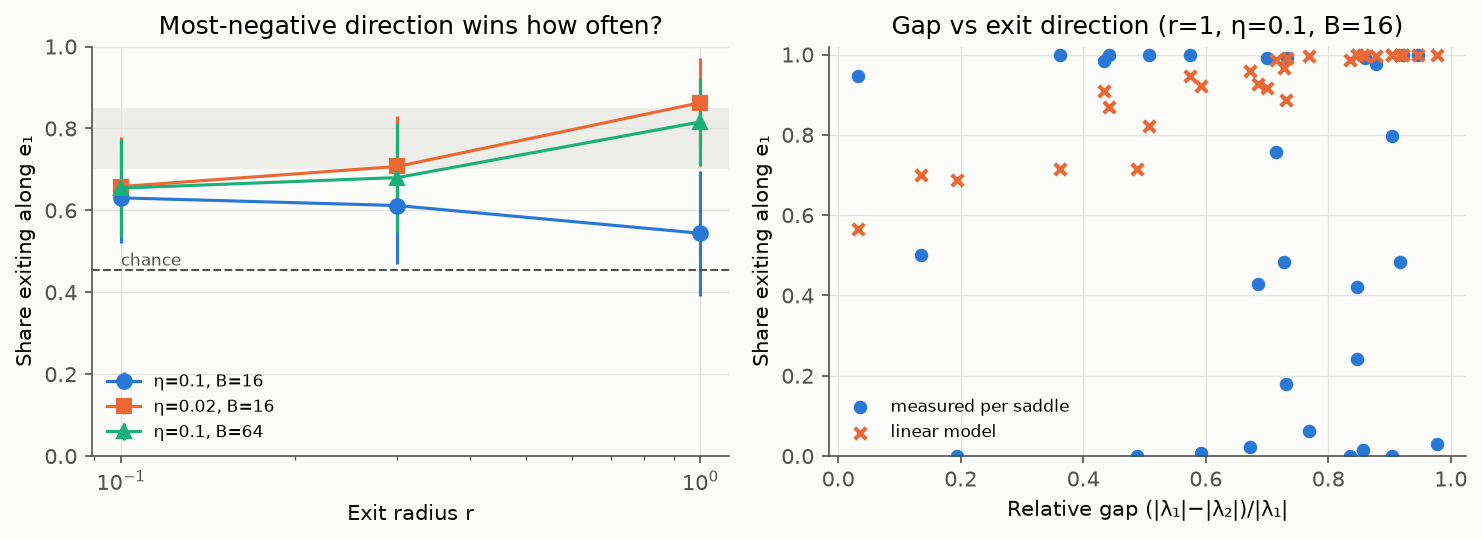
\includegraphics[width=0.95\linewidth]{figures/fig6_saddles.png}
    \caption{Saddle exit direction. \figleft{} Share along $\etop$ against exit radius at three noise levels. The gray band is the hypothesized 70--85\%. \figright{} At high noise and $r=1$, measured per-saddle shares (blue) split between near 0 and near 1 with no relation to the gap, while the linear model (orange) predicts near 1 for most saddles.}
    \label{fig:saddles}
\end{figure}

At low noise the linear model of \eqref{eq:linear} is close (TV 0.13), and curvature matters more than noise projection (noise-only TV 0.30).
At high noise, the model misses.
One third of saddles have an $\etop$ share below 20\%, though the model predicts a median of 0.98.
Per-saddle outcomes stay reproducible anyway, with modal share 88\%.
So exit there is near-deterministic along a non-$\etop$ direction, which random linear growth cannot produce.
Plausible causes are systematic noise-induced drift, or curvature that changes as thermal displacement moves the replica off the saddle.
We tested neither.
